\chapter{Concepts de base}

\section{Introduction}

Les dernières années ont connu un avancement important dans la construction des
machines intelligentes qui ont la capacité d'assister ou de remplacer les
êtres humains pour accomplir plusieurs tâches qui prennent beaucoup de temps ou
qui sont très difficiles.

Ces machines sont dotées de capteurs qui leur donnent la possiblité de percevoir
les différentes caractéristiques des environnements où elles fonctionnent. Un
exemple de ces capteurs peut être une camera qui prend continuellement des photos.
Elles sont équipées aussi de parties mobiles qui leur permettent
d'interagir avec leur environnement. De plus, elles doivent
être programmables afin de pouvoir les affecter à des tâches précises.

Mis à part le côté matériel, les machines qui peuvent remplacer l'homme disposent
de notions d'intelligence artificielle représentées par l'implémentation d'une ou
plusieurs techniques issues de cette science, comme les techniques de la
recherche dans un espace de solutions et celles de l'apprentissage automatique.

Nous commençons ce chapitre par la présentation de la robotique, suivi par
la définition de quelques notions de la vision artificielle, et nous terminons
par l'exposé des techniques d'apprentissage automatique.

\section{La robotique}

C'est une discipline qui fait partie de la mécanique, de l'électrique, et de
l'informatique en même temps. Elle s'intéresse à la conception, à la
construction et au fonctionnement des \keyword{robots}, ainsi à la création
des systèmes informatiques qui les contrôlent.

\subsection{Le robot}

Le mot \keyword{robot} réfère à un agent électromécanique autonome ou
semi-autonome, guidé par un programme informatique ou un circuit électronique.

Il existe plusieurs types de robots répondant à différents fonctions. Nous
citons les plus importants.

\begin{itemize}
  \item Les robots mobiles ont la possibilité de se déplacer dans leur
  environnement pour accomplir leurs tâches.
  \item Les robots industriels sont construits à partir de bras jointés et
  sont utilisés dans les lignes de production.
  \item Les robots de service ont un rôle proche de celui des robots
  industriels, sauf qu'ils sont utilisés pour fournir des services autres que
  la production.
  \item Les robots éducationnels sont utilisés comme des assistants
  éducationnels pour les enseignants afin d'aider les élèves à mieux comprendre
  des concepts mathématiques, physiques, électroniques et programmatifs.
\end{itemize}

La structure d'un robot comporte trois éléments du point de vue construction.

\begin{description}
  \item[Sur le plan mécanique,] tous les robots sont conçus pour leurs
  permettre d'accomplir leurs tâches. Cette construction dépend du type de la
  machine et de l'environnement où elle fonctionne. Elle définit la forme
  extérieure et la structure interne du robot.
  \item[Sur le plan électrique,] un robot a besoin de composants
  électriques qui lui offrent la possibilité de
  contrôler son corps mécanique et de capturer les caractéristiques de son
  environnement.
  \item[Sur le plan programmatif,] chaque robot doit avoir un certain
  niveau de programmation qui le permet de
  savoir comment réaliser une opération ou prendre une décision. Cette
  programmation peut être réalisée par une combinaison des circuits intégrés dans
  les cas simples, ou à l'aide d'une série d'instructions exécutées sur un
  microprocesseur dans les cas les plus complexes.\cite{wikipediaRobotics}
\end{description}

\subsection{Les composants électroniques}
Chaque circuit électronique est constitué d'un nombre de \keyword{composants}
réalisant la tâche de ce circuit à l'aide d'une source d'énergie. Ces composants
ont des \keyword{terminaux} qui permettent leur connexion à travers des
\keyword{câbles}. Chaque composant a un rôle précis dans le circuit qui peut être
un traitement logique, une transformation du signal, ou la protection d'autres
composants. Ils sont classés en trois types : \keyword{passifs},
\keyword{actifs} et \keyword{électromagnétiques}.\cite{wikipediaElectronicComponent}

\begin{description}
  \item[Les composants passifs] ne manipulent pas le signal électrique
  et ne modifient que l'intensité ou la tension électrique. Parmi ces composants
  on trouve les résistances et les condensateurs.
  \item[Les composants actifs] manipulent le signal électrique pour
  effectuer leurs traitements. Ils sont fabriqués principalement de matériaux
  semi-conducteurs. Les diodes, les transistors et les circuits intégrés sont
  considérés comme des composants actifs.
  \item[Les composants électromagnétiques] transforment l'énergie de la
  forme électrique vers la forme magnétique ou l'inverse. Les relais, les
  moteurs électriques et les transformateurs sont des composants électromagnétiques.
\end{description}

\begin{figure}[H]
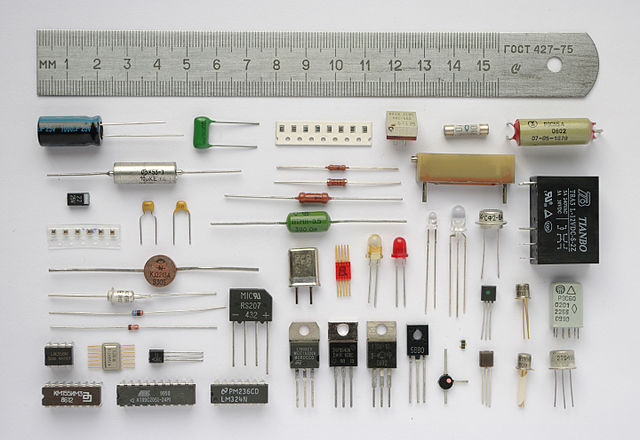
\includegraphics[width=\textwidth]{Componentes}
\caption{Des composants électroniques}{\cite{commonsComponents}}
\end{figure}

\subsection{Les modules électroniques}
Un module est un circuit fabriqué de plusieurs composants qui sont imprimés sur
une carte. Il représente une unité dédiée à réaliser une tâche donnée. Chaque
module contient tous les composants électroniques nécessaires pour son
fonctionnement ainsi que des connecteurs assurant son branchement avec les
autres modules. Dans les petits circuits, ils sont alimentés par un courant
direct qui a une tension de $5$v ou de $3.3$v selon le type du module, bien
que d'autres peuvent supporter une tension de $12$v.

\begin{description}
  \item[Le microcontrôleur] est un module électronique programmable ayant une
  capacité limitée de traitement de données. Il inclut un microprocesseur, une
  mémoire centrale et une mémoire secondaire à lecture seule mais reinitialisable.
  Il peut lire les données reçues des autres modules et leurs envoyer des commandes
  pour contrôler leur fonctionnement à travers ses ports. Chaque système embarqué
  contient au moins un microcontrôleur. La puissance du microcontrôleur
  dépend de son architecture, de sa taille d'instructions et aussi de la fréquence
  de son horloge.
  \item[Les capteurs] sont des modules qui permettent d'obtenir des données sur
  l'environnement sous forme d'un signal électrique numérique ou analogique.
  Parmi ces capteurs, on trouve les capteurs de la température qui permettent de
  mesurer le degré de température de l'environnement où ils se trouvent quand ils
  sont activés par un signal.
  Il y a aussi les capteurs ultrasoniques permettant d'envoyer un ultrason et
  d'en attendre la réception.
  Il sont utilisés fréquemment pour le calcul de la distance en mesurant le
  temps écoulé entre l'envoi et la réception du signal en connaissant la vitesse
  du son dans l'environnement.
  \item[Les moteurs] sont les composants qui transforment l'énergie électrique en
  mouvement mécanique. Ils tournent dans un seul sens et à une vitesse qui
  sont déterminés respectivement par le sens et l'intensité du courant électrique.
\end{description}

\section{Vision artificielle}

La vision artificielle est une branche de l'informatique qui s'intéresse aux
techniques de la compréhension d'une scène par un ordinateur. Différentes
techniques issues de la géométrie et de l'intelligence artificielle ont été
développées dans ce domaine afin de résoudre des problèmes liées à la vision,
comme la reconnaissance, la localisation des objets et la description de
la scène. Ces techniques sont appliquées sur des images d'une scène.

\subsection{L'image}

Dans la vision par ordinateur, une image est une matrice multidimensionelle.
Généralement elle est de deux dimensions (hauteur et largeur) si
elle est monochrome. Dans les autres cas, elle est de trois dimensions, la troisième
dimension étant le nombre de \keyword{canaux}.

Un canal est directement relié à l'espace de couleurs de l'image.
Pour une image ordinaire, il en existe trois correspondant aux couleurs de base
de l'espace RGB (Rouge, Vert, Bleu). \`A noter que les images ayant trois
canaux ne sont pas toutes des images RGB. A titre d'exemple, certaines utilisent
l'encodage HSV (Hue, Saturation, Value) qui sépare la teinte de la luminosité et
de la saturation. Certaines images contiennent l'information de la transparence
et donc ont un canal supplémentaire connu sous le nom de canal \keyword{Alpha}.
Comme on l'a dit précédemment, il existe des images qui ont quatre canaux sans
avoir la transparence, comme celles utilisant l'espace de couleurs CMYK
(Cyan, Magenta, Yellow, Black) qui définie chaque point comme une
combinaison du noir avec trois autres couleurs : le cyan, le magenta et le jaune.
Ces couleurs sont utilisées pour l'impression.

Vu que les images sont des matrices, toutes les opérations matricielles usuelles
(comme l'addition, la multiplication, etc) s'appliquent mais sans déborder des
intervalles des canaux. Ces intervalles sont définis généralement sur des
valeurs entre $0$ et $255$.

Les opérations matricielles classiques sont peu utilisables pour le traitement
d'images mais d'autres ont été créées pour ce besoin. L'une des opérations les
plus utilisées est \keyword{la convolution}.

\subsection{La convolution}

C'est une opération de base qui consiste à effectuer la somme de la multiplication
élémentaire entre une partie de l'image et la matrice de la convolution qui est
généralement carrée et de taille beaucoup plus petite que celle de l'image.
Elle est appelée \keyword{noyau} ou \keyword{filtre} de la convolution.

Au début, le filtre opère sur la partie supérieure gauche de l'image pour
calculer la nouvelle valeur du pixel concerné. Il sera
par la suite déplacé toute au long de l'image pour générer les autres valeurs
qui vont former ensemble une autre image dont le contenu dépend des valeurs du
filtre.

\begin{figure}[h]
\begin{subfigure}{0.49\textwidth}
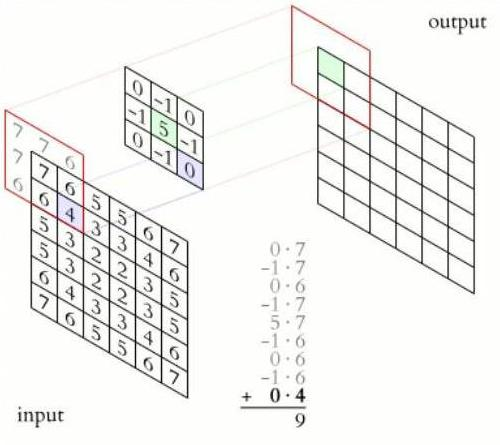
\includegraphics[width=\textwidth]{Conv1}
\end{subfigure}
\hfill
\begin{subfigure}{0.49\textwidth}
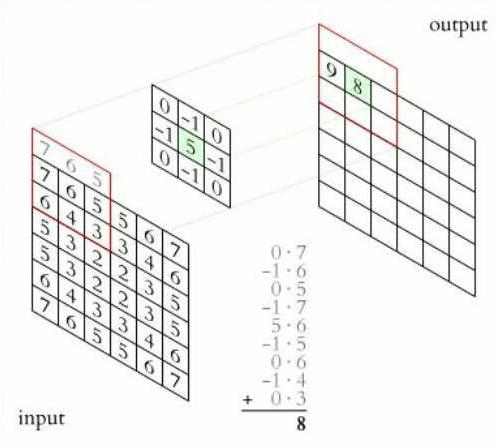
\includegraphics[width=\textwidth]{Conv2}
\end{subfigure}
\caption{La convolution}{\cite{commonsConvolution}}
\end{figure}

\section{Apprentissage automatique}

L'apprentissage automatique est une filière de
l'intelligence artificielle qui s'intérresse aux techniques de conception des
modèles ayant la capacité d'apprendre à réaliser une tâche sans les programmer
explicitement. Ces modèles sont des fonctions paramétrées dont les paramètres
peuvent être changés par un \keyword{entraînement} en utilisant les données
disponibles. Une fois que le modèle est entraîné, il sera capable d'opérer sur
de nouvelles données qui n'ont pas été vues lors de l'apprentissage.

Il y existe de nombreuses méthodes, chacune appartenant à
une des trois classes :
\keyword{l'apprentissage par renforcement} (par récompenses),
\keyword{l'apprentissage non supervisé} et
\keyword{l'apprentissage supervisé}.

\subsection{Apprentissage par renforcement}

Dans ce mode, chaque fois que le modèle génère un résultat, il sera informé
si son résultat est acceptable ou non. Dans le cas non favorable, il modifiera
ses paramètres pour essayer d'améliorer la solution. Le résultat d'une action
prise par le modèle n'est jamais connu avant l'essai. Parmi les algorithmes de ce
mode on trouve le \keyword{Q-learning}.

\subsection{Apprentissage non supervisé}

C'est le mode qui permet de trouver une structuration interne pour des données
non étiquetées. Les approches de ce mode tentent de distribuer les données sur
des ensembles générés lors de l'apprentissage selon des critères qui diffèrent
en fonction du type d'algorithme utilisé. Plusieurs algorithmes ont été
développés dans ce mode comme \keyword{K-means}.

\subsection{Apprentissage supervisé}

C'est un mode permettant de trouver une approximation d'une fonction en utilisant
les données avec les résultats attendus de cette fonction. Un modèle approximant
la fonction sera généré en utilisant une des techniques de ce mode.
Il peut être appliqué sur des problèmes de régression dont l'objectif est
d'approximer une fonction continue, ou bien sur des problèmes de classification
dont le but est de trouver la bonne classe pour une instance.

Cet apprentissage peut être considéré comme un problème d'optimisation
dans un espace multidimensionel formé de valeurs d'attributs discrètes ou
continues. Le but est de minimiser la valeur d'erreur calculée par une
\keyword{fonction de coût} qui estime la distance entre les valeurs retournées
par le modèle et les valeurs attendues.

Parmi les techniques les plus utilisées dans ce mode on trouve
\keyword{la régression linéaire}, \keyword{la régression logistique},
\keyword{les machines à vecteurs de support},
\keyword{les classifieurs bayésiens naïfs} et
\keyword{les réseaux de neurones artificiels} auxqueles nous avons recours dans
ce projet.

Les réseaux de neurones artificiels est une technique inspirée du cerveau humain.
Son architecture est composée de plusieurs \keyword{couches} dont chacune
contient plusieurs unités de calcul dites \keyword{perceptrons}.

\begin{figure}[h]
\begin{center}
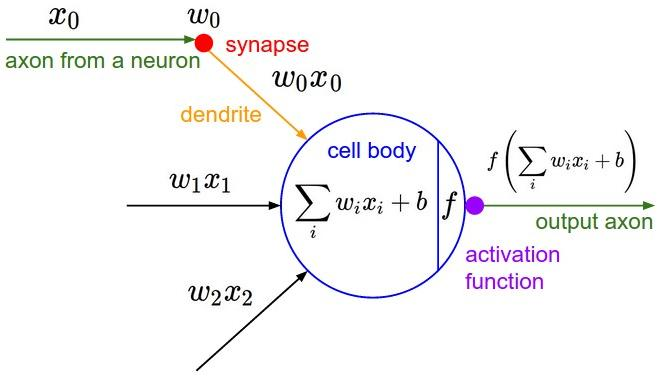
\includegraphics[width=0.5\textwidth]{neuron_model}
\caption{Le schéma d'un perceptron}{\cite{karpathy2016cs231n}}
\end{center}
\end{figure}

Chaque perceptron est une composition d'une somme de
produits scalaires avec une \keyword{fonction d'activation} qui permet
généralement d'émettre une valeur comprise entre $0$ et $1$.
Il existe des connexions entre les perceptrons dont le nombre et le type dépend
du type du réseau.

\begin{figure}[h]
\begin{center}
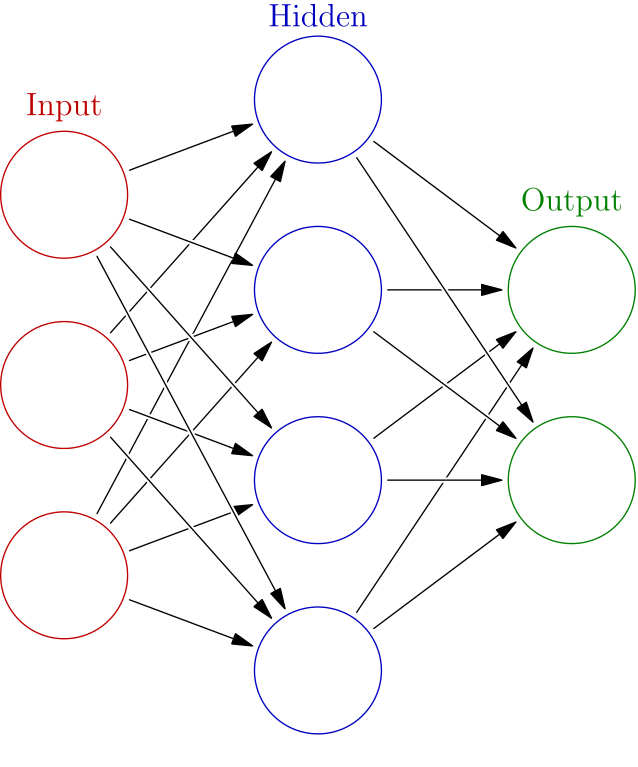
\includegraphics[width=0.5\textwidth]{ColoredNeuralNetwork}
\caption{Un réseau de neuronnes artificiel}{\cite{commonsANN}}
\end{center}
\end{figure}

Il y a plusieurs types de réseaux de neurones, comme
les réseaux d'alimentation vers l'avant, \keyword{les réseaux récurrents}, etc,
chaque type étant adapté à un type de problèmes.
Dans les problèmes liés aux images, le type préféré est celui des
\keyword{réseaux convolutionels} dont nous nous servirons et que nous détaillons
au point suivant.

\section{Les réseaux convolutionels}

Ils sont une modification des réseaux d'alimentation vers l'avant qui consiste à
traiter des régions spaciales de la donnée au lieu de considérer sa globalité.
Ils se composent de trois couches de types différents :
\keyword{les couches convolutionelles},
\keyword{les couches de regroupement (mise en commun)} et
\keyword{les couches entièrement connectées (denses)}.

\begin{figure}[h]
\begin{center}
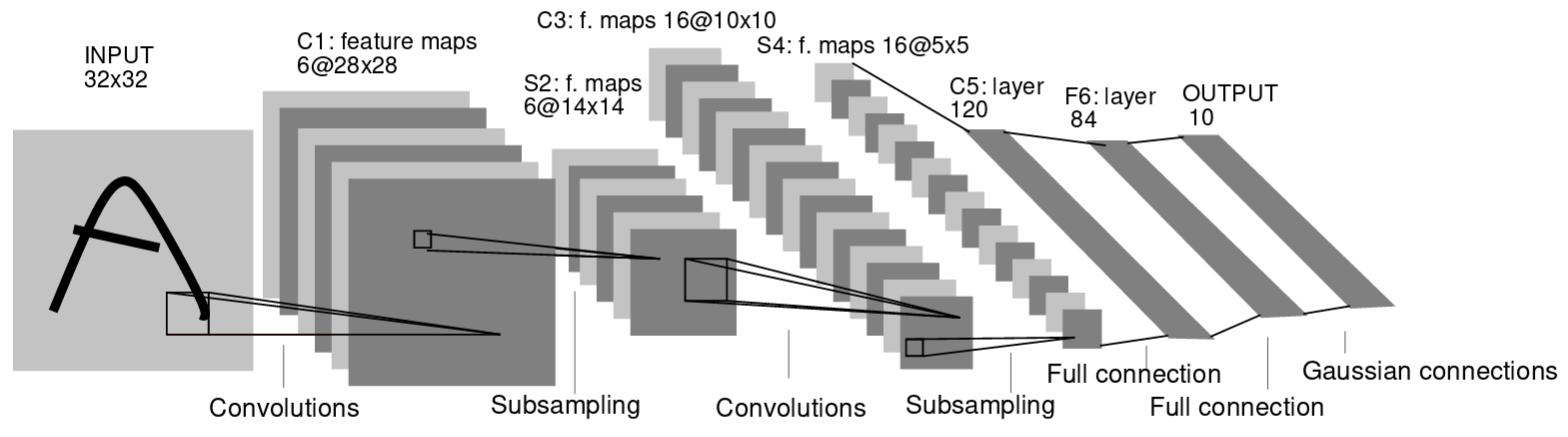
\includegraphics[width=\textwidth]{LeNet-5}
\caption{Le réseau convolutionel le plus ancien : LeNet-5}{\cite{lecun1998gradient}}
\end{center}
\end{figure}

\subsection{Couches convolutionelles}

Dans une couche de convolution, chaque perceptron est relié seulement à un petit
sous-ensemble de perceptrons de la couche précédente. Cet ensemble représente
une région rectangulaire dans une image. L'image peut être l'originale ou
bien la résultante des opérations des couches précédentes. La fonction générant
chaque région est appelée le \keyword{filtre}. Ce type de couches est généralement
placé au début et au milieu du réseau.

Chaque couche convolutionelle nécessite des hyperparamètres qui doivent
être fixés dans la conception : la taille spatiale du filtre $F$ et la
profondeur du filtre $K$, le pas de la convolution $S$, le rembourrage par zéro
$P$, et la fonction d'activation.

\begin{description}
  \item[La taille spatiale du filtre $F$] sert à
  spécifier le nombre d'entrées pour chaque perceptron,
  \keyword{la profondeur du filtre $K$} spécifie
  le nombre de matrices de poids partagés.
  \item[Le pas de la convolution $S$] est la différence entre le bord d'un
  filtre et le même bord du filtre du perceptron successif.
  \item[Le rembourrage par zéro $P$] permet d'entourer
  l'entrée par des pixels nuls avant d'appliquer la convolution pour maintenir
  sa taille.
  \item[La fonction d'activation] qui, à la sortie de chaque couche, permet grâce
  à une fonction mathématique de modifier les valeurs avant de les transmettre à la
  couche suivante.
\end{description}

\subsection{Couches de regroupement}

Le rôle de ces couches est de réduire la taille spatiale du résultat des couches
précédentes en gardant l'information essentielle. Cette opération est souvant
appliquée en utilisant la valeur maximale entre les pixels ou par le calcul de
la moyenne. Ces couches sont généralement placés après les couches
convolutionelles.

Les hyperparamètres requis pour cette couche sont les mêmes que ceux des couches
convolutionelles, auxquelles il faut ajouter la fonction de regroupement
(maximum ou moyenne).

\begin{figure}[h]
\begin{center}
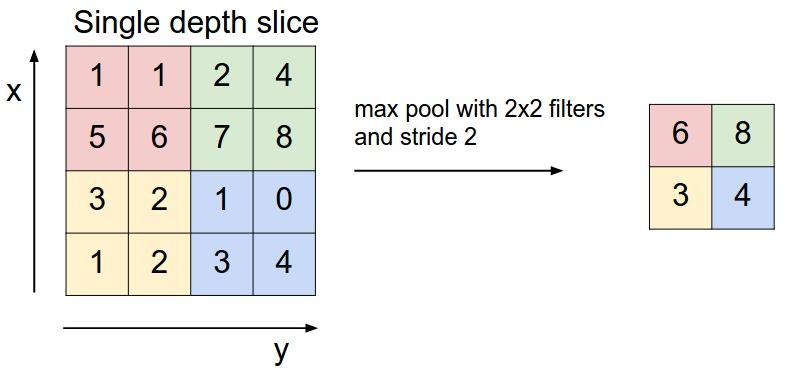
\includegraphics[width=0.75\textwidth]{maxpool}
\caption{L'opération de regroupement par le maximum}{\cite{karpathy2016cs231n}}
\end{center}
\end{figure}

\subsection{Couches entièrement connectées}

C'est le type classique des couches dans un réseau de neurones artificiels. Ils
sont les mêmes que ceux utilisées dans les réseaux d'alimentation vers l'avant.
Chaque perceptron dans ce type est connecté à tous les perceptrons de la couche
précédente. Ces couches sont utilisées à la fin du réseau.

Les hyperparamètres nécessaires pour ce type sont :

\begin{itemize}
  \item le nombre de perceptrons $K$,
  \item la fonction d'activation.
\end{itemize}

\section{Conclusion}

Ce chapitre a été consacré aux notions de robotique, de vision artificielles
et d'intelligence artificielle requises pour la compréhension du sujet.
D'abord, nous avons présenté les types de robots et les composants qui assurent leur
fonctionnement. Ensuite, nous avons défini les images de la perspective
informatique et l'opération de la convolution. Enfin, nous avons présenté le
domaine de l'apprentissage automatique en insistant sur les réseaux de
neurones artificiels convolutionels.

Le chapitre suivant sera reservé pour la présentation de quelques projets antérieurs
de chercheurs qui ont travaillé sur l'estimation de distances à partir des images.
Leur approches respectives seront exposées avec les explications nécessaires avant
d'entamer la présentation détaillée de notre propre réalisation.
